\chapter{Conclusion}
\label{chapter:conclusion}

This work showed how PCG is important in game design and how the price of game development has been increasing throughout the years, it proposed the development of a PCG system to generate good cave-like maps and finally it evaluated this system through a survey.

One of the biggest challenges faced was the research for criteria on what makes a good map, that can be seen on Section \ref{sec:goodmap} of Chapter \ref{chapter:proposal}. Most of the work we found focused on video-game \emph{levels}, which contain more elements like enemies and treasures. Due to this difficulty we decided to also include metrics from the ARCS model, taking inspiration from \cite{carvalho:2016}, and adapted them, since they are normally used to measure motivation in learning. In this sense, the evaluation method for generated maps proposed on this work can be reused by others.

The creation of the system required knowledge from different areas and the use and adaptation of many algorithms. The system had many user-defined parameters which is a positive in map generation, since a larger variety of maps can be created. Even though the work focused on cave-like maps, by changing the used tiles the system can generate maps like forests, open fields, rivers etc. Figure \ref{fig:river} shows a procedurally generated river, created with the use of the system.

\begin{figure}[h]
    \caption{River generated by the system.}
    \centerline{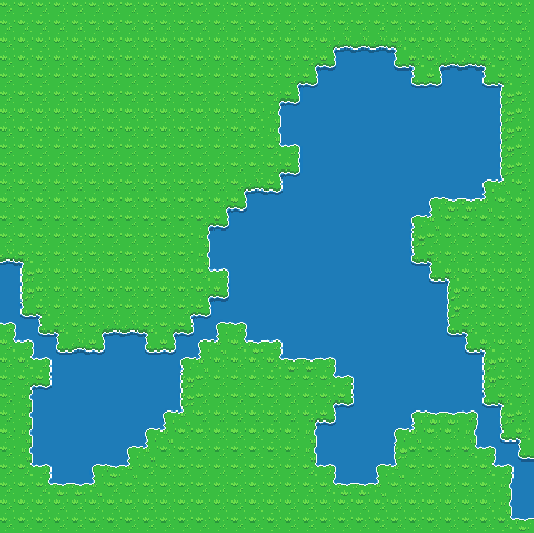
\includegraphics[width=6cm]{images/river.png}}
    \legend{Source: Image provided by author}
    \label{fig:river}
\end{figure}

The survey was answered by 163 participants, most of them from the age group that composes the average gamer, and most of them with familiarity to 2D top-down games. From the 12 questions, 9 achieved satisfactory results and 3 did not. Out of these results we found that the generated maps were successful in giving motivation. We also found that, even thought the structure of the maps resemble natural caves, the maps were not found to be much similar to 2D representations of real caves.

Finally, as a future works, the system could be turned into an Unity tool, that can then be used to create full games. The generation of rivers can be expanded on, by comparing them to real-life rivers and evaluating with a similar survey. The generation of maps can be changed to a level-generator, where the system wouldn't only generate the map but also place enemies, treasures, hidden passages etc.